\documentclass{stdlocal}
\begin{document}
\section{SIMD-Capable Processors} % (fold)
\label{sub:simd-capable_processors}

  According to \textcite[\ppno~10-11]{hennessy2019}, in the year 1966, Flynn classified parallel architectures of computers with respect to their data-level and task-level parallelism.
  Based on this classification, a conventional uniprocessor has a single instruction stream and single data stream, also known as single instruction single data (SISD) architecture \autocite[\ppno~509-510]{patterson2014}.
  The single instruction multiple data (SIMD) architecture exploits data-level parallelism by applying the same operations to multiple items of independent data at the same time \autocite{hennessy2019} which, from the programmer's perspective, is close to the SISD mode of operation \autocite{patterson2014}.
  In contrast to the multiple instruction multiple data (MIMD) architecture, SIMD only has to fetch one instruction to launch several data operations potentially reducing the power consumption.
  The application of SIMD ranges from matrix-oriented algorithms in scientific computing to media-oriented image and sound processing, as well as machine learning algorithms \autocite[\ppno~10-11]{hennessy2019}.
  Modern Intel processors typically provide SIMD utilities through special vector registers and a richer instruction set, like the Streaming SIMD Extensions (SSE) and the Advanced Vector Extensions (AVX) \autocite{intel-intrinsics-guide,fog2019a,fog2019b,fog2019c,fog2019d,fog2019e}.
  At the same time, MIMD utilities are implemented through multiple processor cores and multithreading.
  In a modern processor, SIMD and MIMD are orthogonal features of its design and can therefore be discussed independently.
  Hence, we will not focus on the exploitation of the MIMD architecture.
  To be able to design and implement vectorized algorithms for an SIMD architecture, we have to explain how data-level and instruction-level parallelism can be used to raise the performance of a computer program.
  % Vectorization techniques can be conceptualized by the architecture of modern SIMD-capable multiprocessors and their instruction sets.
  Especially the knowledge of typical instructions will make the design of a new API and its application to Monte Carlo simulations clear.
  Therefore, we will briefly introduce the fundamentals of computer architecture and refer to \textcite{patterson2014} and \textcite{hennessy2019} for a more detailed observation.

  \subsection{Fundamentals of Computer Architecture}
    The Von Neumann architecture still describes the basic organization of a modern computer.
    Besides external mass storage, like hard disk drives (HDDs), and input/output (IO) mechanisms, the model uses a central processing unit (CPU), also called the processor, to execute instructions from a computer program, and memory to store the respective data and instructions \autocite{hennessy2019}.
    Today, both, data and instructions, are encoded as binary numbers with fixed length which has proven to make the building and functioning of a computer much more efficient \autocite{patterson2014}.

    \begin{figure}
      \center
      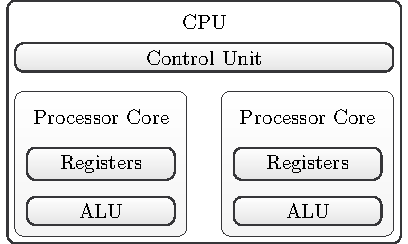
\includegraphics[width=0.5\textwidth]{figures/cpu_components.pdf}
      \caption[Hierarchical Order of CPU Components]{%
        The figure shows the basic components of a typical CPU with multiple processing cores in an hierarchical order.
        There is only one control unit which is handling communication between different cores by coordinating the execution of program instructions.
        Every processor core employs its own registers and ALUs to provide an MIMD architecture.
      }
      \label{fig:cpu-components}
    \end{figure}
    The processor in general consists of an arithmetic logic unit (ALU), a small number of registers and a control unit.
    The ALU performs arithmetic and logic operations and stores its results in registers.
    These registers also supply the operands for ALU operations.
    To fetch program instructions from memory and executing them, the control unit directs the coordinated operations of the ALU, registers and other components.
    Today, nearly every processor consists even of multiple processing cores each connected by a global control unit and containing its own registers and ALUs to provide an MIMD architecture.
    In figure \ref{fig:cpu-components}, all the named components are shown schematically in a hierarchy to support the understanding.
    Here, we will focus on a single processing core.
    The set of instructions a processing core is able to execute is called its architecture.
    Usually, processor architectures provide commands to move data between memory and CPU registers and simple arithmetic and logic operations, like addition and multiplication of integral or floating-point numbers, to actually compute results of algorithms.
    \autocite{hennessy2019,patterson2014}

    Memory can be described as a finite sequence of bits, whereby each bit anytime represents either the value $0$ or $1$.
    Eight bits are grouped into a byte and enumerated with a natural number starting from zero.
    These numbers are called memory addresses and make it possible to specify the location of variables in memory.
    This basic interpretation is visualized in figure \ref{fig:memory}.
    Fetching instructions from memory or transferring data between the CPU and memory, therefore requires the usage of those memory addresses to be able to reference data in the sequence of bytes.
    Each byte can be altered by program execution through storing instructions.
    \autocite{patterson2014}
    \begin{figure}[H]
      \center
      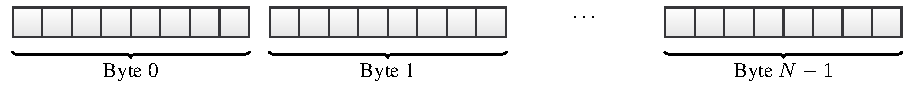
\includegraphics[width=0.95\textwidth]{figures/memory.pdf}
      \caption[Memory Structure]{%
        This figure visualizes memory with $N\in\setNatural$ bytes as a sequences of bits where each byte can be referenced by its memory address.%
      }
      \label{fig:memory}
    \end{figure}
    Because physically there is no possibility to provide an unlimited amount of fast memory, computer designers found a more economical solution.
    In the majority of cases, faster memory means reduced storage capabilities and vice versa.
    Hence, memory is built to be a hierarchy of several levels --- each smaller, faster, and more expensive per byte than the next lower level, which is farther from the processor.
    Interleaving levels are called caches and with caching we mean the process of loading data into the next cache level.
    If the processor wants to load some data from memory which cannot be found in the first level cache, data has to be fetched from a lower level in the hierarchy.
    This is called a cache miss.
    If on the other hand the data can be found in the cache, it can be directly used by the higher level cache or the processor itself.
    We call this a cache hit.
    A cache miss introduces a so-called miss penalty to the memory access time and should therefore be avoided to reduce the latency for fetching instructions and data.
    Figure \ref{fig:memory-hierarchy} shows a schematic view of a usual memory hierarchy found in today's laptops and desktop computers.
    In modern processor architectures, like the Kaby Lake microarchitecture from Intel, each processing core of the CPU features its own level one cache which is further split into an instruction cache and a data cache \autocite{intel-kaby-lake}.
    This reduces the overall complexity of level one caches and as a result decreases the cache access time.
    \autocite[\ppno~78-83]{hennessy2019}
    \begin{figure}
      \center
      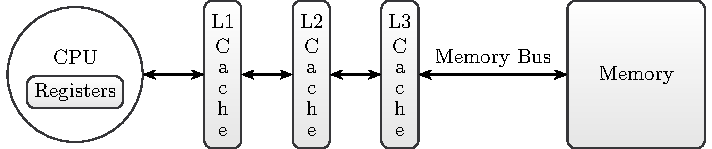
\includegraphics[width=0.95\textwidth]{figures/memory_hierarchy.pdf}
      \caption[Memory Hierarchy Scheme]{%
        The figure shows a scheme of the non-persistent part of the memory hierarchy for a modern laptop or desktop computer.
        Modeled after \textcite[\pno~79]{hennessy2019}.
      }
      \label{fig:memory-hierarchy}
    \end{figure}

    A variable in the memory is accessed most efficiently if it is stored at a memory address which is divisible by the size of the variable.
    This is typically called alignment.
    Especially for SIMD instructions, a certain alignment is even required.

    Executing an instruction is done is several stages.
    \begin{enumerate}
        \item Fetch instruction from memory.
        \item Read registers and decode the instruction.
        \item Execute the actual operation.
        \item Write the result into a register.
    \end{enumerate}
    To speed up this process, in nearly all modern CPUs a pipeline is used.
    The number of stages an instruction needs until it is finished is called its latency.
    Using a pipeline does not reduce the latency of an instruction but increases its throughput, the number of instructions which are computable per CPU cycle, due to parallel execution of the different stages.
    It is therefore a form of instruction-level parallelism.

    \begin{figure}
      \center
      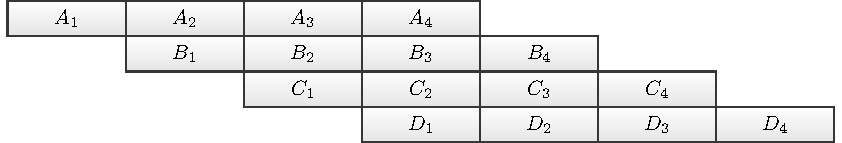
\includegraphics[width=0.95\textwidth]{figures/pipeline.pdf}
      \caption[Pipeline Structure]{%
        This figure shows the functioning of a pipeline.
      }
      \label{fig:pipeline}
    \end{figure}
    The theoretical performance of the CPU pipeline is reduced if it has to be stalled.
    These situations, also known as hazards, happen due hardware resource conflicts, data dependencies and control instructions, like branches.
    To handle control instructions and especially branches much more efficiently, the CPU uses branch prediction.
    The processor tries to guess the outcome of the branch condition to keep the pipeline filled.
    Should the estimated value proven to be wrong the pipeline has to be stalled and cleared.
    This process is called branch miss and introduces an execution time penalty.
    Hence, we will strive for branchless code or for easy-to-predict branches if we have to insert them.

    \begin{figure}
      \center
      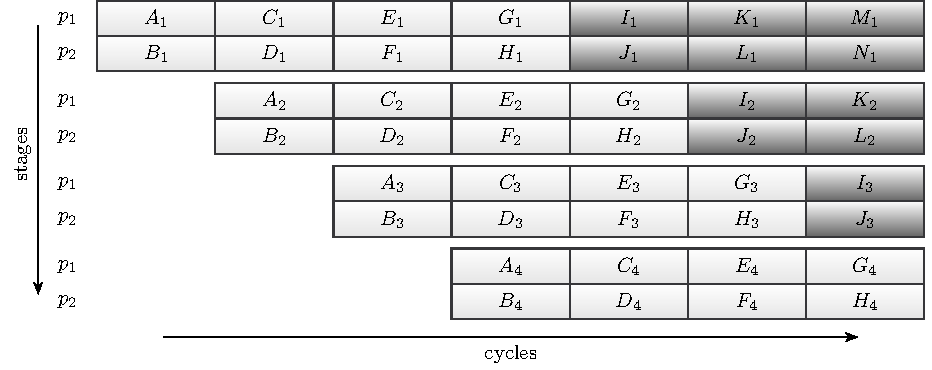
\includegraphics[width=0.95\textwidth]{figures/multiple_unit_pipeline.pdf}
      \caption[Multiple Unit Pipeline Structure]{%
        This figure shows the functioning of a pipeline.
      }
      \label{fig:multiple-unit-pipeline}
    \end{figure}
    Another variant of instruction-level parallelism is to decrease the cycles per instruction (CPI) to less than one.
    A processor typically uses more than computation unit to achieve this.

    For data-level parallelism, we want to focus on single instruction multiple data (SIMD) architectures.
    Intel CPUs establish this feature by using so-called vector registers.
    Vector registers contain more than one value at the same time.
    One operation is then performed on all contained elements.

  \subsection{Usage in C++} % (fold)
  \label{sub:usage_in_c_}
    For Intel processors, we are able to use Intel intrinsics to force the usage of vector operations and vector registers.
    The alignment can automatically forced by the compiler or manually set by the programmer.
    Tables for latencies and throughput can be found by intel and agner fog.
    For certain compilers certain compiler flags have to be used.
    According to agner fog, striving for compatibility means we have to require certain instruction set features, like SSE or AVX or FMA.
    Typically, compilers use an automatic vectorization approach.
    But this is only possible if there are no data dependencies.
    Most of the time code has to be adjusted.
    Therefore we tend to do this manually.
  % subsection usage_in_c_ (end)
% section simd-capable_processors (end)
\end{document}